\documentclass{standalone}
\usepackage{xcolor,amsmath,amssymb,amsfonts}
\usepackage{fontspec}
\usepackage[T1]{fontenc}
\usepackage[tt=false, type1=true]{libertine}
\usepackage[libertine]{newtxmath}

\usepackage{tikz}
\usetikzlibrary{arrows.meta}
\definecolor{red}{HTML}{c63a44}
\begin{document}

$$
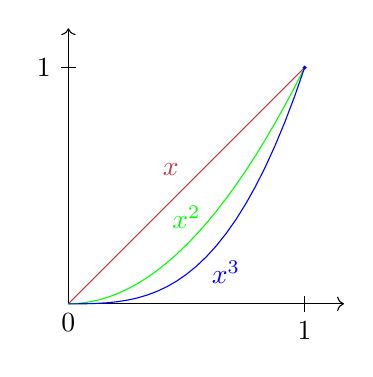
\begin{tikzpicture}
    \draw[->] (0, 0) node[anchor=north]{0}-- (0, 3.5);
    \draw (0.1, 3) -- (-0.1, 3) node [anchor=east, align=right] {1};
    \draw[->] (0, 0) -- (3.5, 0);
    \draw (3, 0.1) -- (3, -0.1) node [anchor=north, align=center] {1};
    \draw [red,domain=0:3] plot (\x, \x);
    \node[red] at (1.3, 1.7) {$x$};
    \draw [green, domain=0:3] plot (\x, {3 * pow(\x / 3, 2)});
    \node[green] at (1.5, 1.1) {$x^2$};
    \draw [blue,domain=0:3] plot (\x, {3* pow(\x / 3, 3)});
    \node[blue] at (2, 0.4) {$x^3$};
    \node[circle, fill=blue, draw=blue, inner sep=0.3] at (3, 3) {};
\end{tikzpicture}
$$

\end{document}